% \documentclass{easychair}
\documentclass[EPiC]{easychair}
%\documentclass[EPiCempty]{easychair}
%\documentclass[debug]{easychair}
%\documentclass[verbose]{easychair}
%\documentclass[notimes]{easychair}
%\documentclass[withtimes]{easychair}
%\documentclass[a4paper]{easychair}
%\documentclass[letterpaper]{easychair}

\usepackage{doc}
\usepackage{float}

\newenvironment{packed_itemize}{
\vspace*{-0.5em}
\begin{itemize}
  \setlength{\partopsep}{0pt}
  \setlength{\itemsep}{1pt}
  \setlength{\parskip}{0pt}
  \setlength{\parsep}{0pt}
}{\end{itemize}}

\newenvironment{packed_enumerate}{
\vspace*{-0.5em}
\begin{enumerate}
  \setlength{\partopsep}{0pt}
  \setlength{\itemsep}{1pt}
  \setlength{\parskip}{0pt}
  \setlength{\parsep}{0pt}
}{\end{enumerate}}

% use this if you have a long article and want to create an index
% \usepackage{makeidx}

% In order to save space or manage large tables or figures in a
% landcape-like text, you can use the rotating and pdflscape
% packages. Uncomment the desired from the below.
% \usepackage{rotating}
% \usepackage{pdflscape}

% Make sure to include the slash at the end of the path name
\graphicspath{ {./figures/} }

% Macros
\DeclareMathOperator*{\argmaxA}{arg\,max} % Jan Hlavacek - argmax function

%\makeindex

%% Front Matter
%%
% Regular title as in the article class.
%
\title{Evaluation of Axiom Selection Techniques}
% \thanks{Other people who contributed to this document include Maria Voronkov
%   (Imperial College and EasyChair) and Graham Gough (The University of
%   Manchester).}}

% Authors are joined by \and. Their affiliations are given by \inst, which indexes
% into the list defined using \institute
%
\author{
Qinghua Liu\inst{1}
 \and
Zihao Wang\inst{2}
 \and
Zishi Wu\inst{2}
 \and
Geoff Sutcliffe\inst{2}
% \thanks{Did numerous tests and provided a lot of suggestions}
}

% Institutes for affiliations are also joined by \and,
\institute{
  System Credibility Automatic Verification Engineering Lab of Sichuan Province, Southwest Jiaotong University, China, \email{qhliu@my.swjtu.edu.cn}
\and
   University of Miami, USA, \email{zxw526@miami.edu,zishi@cs.miami.edu,geoff@cs.miami.edu}
 }

%  \authorrunning{} has to be set for the shorter version of the authors' names;
% otherwise a warning will be rendered in the running heads. When processed by
% EasyChair, this command is mandatory: a document without \authorrunning
% will be rejected by EasyChair

\authorrunning{Liu, Wang, Wu, Sutcliffe}

% \titlerunning{} has to be set to either the main title or its shorter
% version for the running heads. When processed by
% EasyChair, this command is mandatory: a document without \titlerunning
% will be rejected by EasyChair
\titlerunning{Evaluation of Axiom Selection Techniques}

\begin{document}

\maketitle
%------------------------------------------------------------------------------
\begin{abstract}
Evaluation of Axiom Selection Techniques
\end{abstract}
%------------------------------------------------------------------------------
\section{Introduction}
\label{Introduction}

``Large Theory'' problems in Automated Theorem Proving (ATP) have been 
defined as having {\em many functors and predicates, and many axioms of 
which only a few are required for the proof of a theorem}.
Large theory problems are mostly found in corpora that contain very many
problems, e.g., the MPTP2078 corpus \cite{AH+14}, the Mizar 40 corpus
\cite{KU15-M40}, and the GRUNGE corpus \cite{BG+19}.
Large theory problems present challenges to ATP systems, because of the
large search space generated by the large number of axioms.
One key to solving large theory problems is selecting a subset of the axioms 
that is adequate for finding a proof. 
There has been significant and successful research on this topic, e.g.,
\cite{PSZG04,SP07,MP09,KC+10,HV11,Kv+12,AH+14,GK15,PU18}.
Many techniques are based on the occurrences of symbols in the formulae,
e.g., the SInE method \cite{HV11} and its derivatives. 
The fact that large theory problems often occur in large corpora makes the
application of machine learning techniques \cite{KB14} viable, e.g., as 
done in the MaLARea system \cite{US+08}.

Evaluation of axiom selection techniques is typically done by:
\begin{packed_enumerate}
\item Choosing a corpus of large theory problems.
\item For each problem in the corpus, selecting a subset of the axioms.
\item Running an ATP system on a reduced problem formed from the selected 
      axioms and the problem's conjecture.
\end{packed_enumerate}
When such experiments are done on large corpora it is necessary to impose
a small time limit when running the ATP system.
In the last step of this proces a proof indicates an adequate selection,
and a countermodel indicates an inadequate selection. 
A timeout provides no information - the selection might be inadequate, or
the selection might be adequate but the reduced problem is too hard because 
too many (unnecessary) axioms were selected and the time limit is too small.
The results are also influenced by the choice of ATP system.

This paper presents metrics for evaluating axiom selection techniques
without having to run an ATP system on the reduced problems.
While the ``proof is in the pudding'' and it is eventually necessary to
evaluate by running an ATP system, the method described in this paper
provides a first-pass evaluation that allows axiom selection techniques to
be rapidly tested and refined.
The approach has the advantage of being independent of a chosen ATP system.
This paper additionally presents some new axiom selection techniques. 
The new techniques the axiom selection built into the Vampire \cite{KV13} and 
E \cite{SCV19} ATP systems, are evaluated using the proposed metrics.

This paper is structured as follows:
Section~\ref{Metrics} describes the evaluation metrics.
Section~\ref{Ours} describes a distance measure between formulae, and
some new axiom selection techniques based on that measure.
Section~\ref{Results} provudes evaluation results.
Section~\ref{Conclusion} concludes.

%------------------------------------------------------------------------------
\section{Selection Metrics}
\label{Metrics}

The principle behind the new evaluation metrics is to compare the selected
subsets of axioms with known adequate sets of axioms.
In this work the MPTP2078 corpus has been used.
The MPTP2078 corpus has two versions of each of the 2078 problems: 
the {\em bushy} (small) versions contain only the Mizar axioms that are
known to be directly used in the proof of the conjecture, and 
the {\em chainy} versions contain all the axioms that precede the conjecture
in the Mizar library order.
The bushy problems contain between N and M axioms, while the chainy versions
contain between N and M axioms.

In order to extract known adequate sets of axioms for each problem, Vampire
and E were run on the problems with a 300s CPU limit.
This produced proofs for NNNN of the bushy problems (KKK by Vampire and JJJ
by E) and MMMM of the chainy problems (KKK by Vampire and JJJ by E).
For the problems solved, the axioms used in proofs were extracted as
known adequate sets of axioms, and new problems formed from those adequate
sets with the corresponding conjectures.
Additionally, in testing the new axiom selection techniques some further
different adequate sets were found, and further new problems created.
This resulted in new problems for NNNN of the bushy problems and
MMMM of the chainy problems.
For some problems multiple adequate sets of axioms were found, resulting in
a total of GGGG new problems for the NNNN bushy problems and a total of
HHHH new problems for the MMMM chainy problems.
The new problems based on the adequate sets have been been used to augment
the MPTP2078 corpus, as the {\em Pruney} problems.
The pruney problems provide adequate known sets of axioms against which
selected sets of axioms can be compared.

GEOFF:
Description of metrics.
Section on selection techniques - cuttion (eg Isabelle) and projection (eg
SInE). 


%------------------------------------------------------------------------------
\section{Our Selection Techniques}
\label{Ours}

GEOFF:
Intro
%------------------------------------------------------------------------------
\subsection{The Symmetric Weighted-average Extended Hutchinson Distance}
\label{QinghuaDistance}

Terms are the most basic structure in the first-order logic. 
A reasonable term metric used for evaluating the term difference can guarantee 
its extended atom and formula metrics perform well to some extent. 
For two arbitrary terms $t_1$, $t_2$, suppose that there exists a substitution 
$\theta$ such that $t_1\theta=t_2$, which reflects the changes from 
$t_1$ to $t_2$. 
In fact, not all two arbitrary terms exist a substitution, and it is thus 
unrealistic to evaluate the term difference by substitutions directly. 
To address the problem, we take the least general generalization $lgg$ of 
terms as a medium to evaluate the term difference. 
Besides, we also propose a way to evaluate the term functional and variable 
difference separately.

Let 
$\theta=\{X_1\mapsto u_1, ..., X_n\mapsto u_n, Y_1\mapsto Z_1, ..., Y_m\mapsto Z_m\}$ 
be an arbitrary substitution, where $u_1$, ..., $u_n$ are functional terms, 
$Z_1$, ..., $Z_m$ are variables, and $X_1$, ..., $X_n$, $Y_1$, ..., $Y_m$ 
are distinct variables. 
functional substitution $\theta_f$ and variable substitution $\theta_v$ are 
defined as:
	\begin{center}
		$\theta_{f}=\{X_1\mapsto u_1, ..., X_n\mapsto u_n\}$, \\
		$\theta_{v}=\{Y_1\mapsto Z_1, ..., Y_m\mapsto Z_m\}$.
	\end{center}
	
Obviously, $\theta_f\cap\theta_v =\emptyset$ and 
$\theta_f\cup\theta_v = \theta$. 
In some special cases, $\theta_f$ or $\theta_v$ may be empty substitution. 
We then put forward two functions $S_f$ and $S_v$, mapping $\theta_f$ and 
$\theta_v$ to real numbers, in which $S_f$ mainly considers the functional 
difference while $S_v$ only takes the variable difference into account. 
$S_f$, $S_v$ are defined as: 
	\begin{align}
		S_{f}(\theta_{f}) &= \sum_{i=1}^{n}occ_{t_1}(X_i)\times(\sum_{f\in F(u_i)}w(f)\times occ_{u_i}(f)); \\
		S_{v}(\theta_{v}) &=\sum_{j=1}^{m}w_{0}\times(log(occ_{t_2}^{+}(Z_{j})-occ_{t_1}^{+}(Y_{j}))).
	\end{align}
Where,
\begin{itemize}
\item $w$ is a weight function that maps every function symbol to a 
      non-negative integer;
\item $w_0$ ($w_0 > 0$) is a constant representing the weight for every 
      variable;
\item $F(t)$ denotes the set of all function symbols appearing in a term $t$;
\item $occ_{t}(s)$ denotes the number of occurrences of a function or variable 
      symbol $s$ in a term $t$;
\item $occ_{t}^{+}(v)$ denotes the number of deep occurrences of a variable 
      $v$ in a term $t$, which takes the depth of $v$ (the number of symbols 
      nested $v$) into consideration. 
      For every occurrence $i$ of $v$, the depth of $v$ is $n_i$ ($n_i\geq$ 0). 
      $occ_{t}^{+}(v)=\sum_{i=1}^{occ_{t}(v)}n_i+occ_{t}(v)$.
\end{itemize}

Given two terms $t_1$ and $t_2$, $t$ is their the least general generalization 
with substitutions $\theta_1$ and $\theta_2$, such that $t\theta_1=t_1$ and 
$t\theta_2=t_2$. 
Based on proposed functions, the term difference function $d_T$ between 
$t_1$ and $t_2$ is defined as:
\begin{align}
	d_T(t_1, t_2) & = \sqrt{[S_f(\theta_{1_{f}})+S_f(\theta_{2_{f}})]^2+[S_v(\theta_{1_{v}})+S_v(\theta_{2_{v}})]^2}.
\end{align}

Compatible atoms can also construct the most general generalization as terms 
do in the same way, thus the $d_T$ can apply to them naturally. 
As for incompatible atoms, we simply think their difference is extremely 
huge due to they cannot be unified. Hence,
\begin{itemize}
	\item if $A_1$, $A_2$ are compatible atoms, $d_A(A_1,A_2)=d_T(A_1, A_2)$;
	\item if $A_1$, $A_2$ are incompatible atoms, $d_A(A_1,A_2)=+\infty$.
\end{itemize}

First-order formulas are the connection of atoms, logical connectives and 
quantifiers. 
Ignoring all the logical connectives and quantifiers, formulas are sets of 
atoms. 
The inference will not happen in such formulas, if all atoms in them are 
incompatible. 
We assert that the more incompatible atoms two formulas have, the less 
similar the formulas are.

Suppose that $F_1$, $F_2$ are two formulas. 
Let $D_1=\{A_1, ..., A_n\}$ and $D_2=\{B_1, ..., B_m\}$, which denote the 
corresponding atom sets, respectively. 
$Penatly=|\{d_A(A_i,B_j) | d_A(A_i,B_j)=(+\infty, +\infty)\}|$ is the number 
of incompatible atom pairs $(A_i,B_j)$ in formulas. 
The formula difference function $d_F$ between $F_1$ and $F_2$ is defined as:
	\begin{align}
		d_F(F_1, F_2) = \frac{n\times m}{Pentaly}\times \sum_{i=1}^n \sum_{j=1}^{m}d_A(A_i, B_j)
	\end{align}

First, we converted a logic problem into a 
fully-connected graph $G = (V, E)$, where each node $v_{i}$ represents a 
logical formulae, and each edge $e_{ij}$ has weight $w'_{ij}$ representing 
the dissimilarity between nodes $v_{i}$ and $v_{j}$. We devised the following 
method to convert each dissimilarity weight $w'_{ij}$ into a similarity 
weight $w_{ij}$:
\begin{align}
w_{ij} = \textrm{max}(0, 
	\argmaxA_{w'_{ij} \subset W} (w'_{ij} \neq \infty) - w'_{ij})
\end{align}

The conversion method consists of three cases:
\begin{itemize}
\item If the dissimilarity weight $w'_{ij}$ is equal to the largest 
dissimilarity weight that is not infinity, or if $w'_{ij} = \infty$, then 
our method will assign a similarity weight $w_{ij} = 0$ to the edge $e_{ij}$.

\item If the dissimilarity weight $w'_{ij} = 0$, then our method will assign 
a similarity weight equal to the largest dissimilarity weight that is not 
infinity (i.e. $\argmaxA_{w'_{ij} \subset W} (w'_{ij} \neq \infty)$).

\item Any dissimilarity weight $w'_{ij}$ between these two extremes will 
yield a similarity weight $w_{ij}$ that is between 
$0$ and $\argmaxA_{w'_{ij} \subset W} (w'_{ij})$.
\end{itemize}

We used the method to convert the dissimilarity matrix $W'$ into a similarity
matrix $W$. 

%------------------------------------------------------------------------------
\subsection{Infinity Cut}
\label{QinghuaInf}

Here, we design a simple conjecture-oriented axiom selection method called 
$infinity$ $cut$, where formula difference function we proposed is used to 
measure the difference between axioms and the given conjecture. 
$infinity$ $cut$ only takes these axioms whose scores of the difference 
to the conjecture are less than $+\infty$ into consideration.

%------------------------------------------------------------------------------
\subsection{Infinity Cut}
\label{QinghuaInf}

2. Qinghua's infinity cut
%------------------------------------------------------------------------------
\subsection{A(nother) Machine Learning Approach}
\label{QinghuaML}

3. Qinghua's ML?
%------------------------------------------------------------------------------
\subsection{Our Selection Techniques}
\label{Zihao}

4. Zihaos way
%------------------------------------------------------------------------------
\subsection{Spectral Clustering with Optimized k}
\label{Zishi}

Spectral clustering is an algorithm used in network science research to
cluster together similar nodes in a graph \cite{vLu07}. 
Given a graph $G = (V, E)$ with an edge weight matrix $W$ such that element
$w_{ij}$ is a measure of similarity between nodes $v_{i} \in V$ and 
$v_{j} \in V$, the algorithm performs two procedures:
\begin{packed_enumerate}
\item Compute a feature matrix $X$ that summarizes the similarity between 
      the nodes in $V$.
\item Applying k-means clustering \cite{} with $X$ as input to partition the 
      nodes into $k$ clusters $K_{1}, K_{2}, ..., K_{k}$.
\end{packed_enumerate}

We ran the spectral clustering algorithm on $W$.
Let $K_{c}$ denote the cluster containing the conjecture, where 
$1 \leq c \leq k$. 

One drawback of the k-means algorithm is that it selects different initial 
centroids each time, and therefore the resulting clusterings vary across 
trials. To address this problem, we devised a way of choosing the initial 
centroids in a deterministic manner:
\begin{itemize}
\item Rank the axioms by degree centrality and select the top $k-1$ axioms.
\item Select the rows of $X$ corresponding to the feature vectors of the
      selected $k-1$ axioms, and the row of $X$ corresponding to the feature 
      vector of the conjecture. 
      Use these $k$ feature vectors as the initial centroids of the k-means 
      algorithm. 
\end{itemize}

Another drawback of the k-means algorithm is that we have no means of 
calculating the optimal number of clusters $k$ beforehand and must therefore 
derive it empirically. To this end, for a logic problem with $N$ logical 
formulae, we tried all values of $k \in [2, N/2]$. We skipped the trivial 
case of $k=1$ because if there is only one cluster, then it contains all the 
axioms and must therefore contain a solution. For each problem, we iterated
through all possible values of $k$ and for each value of $k$, we ran the
spectral clustering algorithm and calculated two metrics: selectivity and 
projection score. We recorded the value of $k$ that yielded the best 
projection score for each problem, and denote that value of $k$ as 
$k_{best}$. This method of axiom selection, which we call 
\textbf{Spectral Clustering with all k's}, becomes computationally 
expensive for large problems with more than a few hundred axioms.

We devised a second method for axiom selection, called 
\textbf{Spectral Clustering with predicted $\mathbf{k_{best}}$}, that uses 
the data collected from the aforementioned process. First, we fitted two
median regression lines, one for the Bushy problems and another for the 
Chainy problems, onto the data of $k_{best}$ versus $N$. This gave us a 
linear model to predict $k_{best}$ for a given problem containing $N$
logical formulae, which we used to obtain for each problem a predicted
$k_{best}$. Finally, we applied each predicted $k_{best}$ on the spectral
clustering algorithm to obtain a selectivity metric and projection score
metric for each problem. The median regression best fit lines are shown 
below.
\begin{figure}[H]
	\centering
	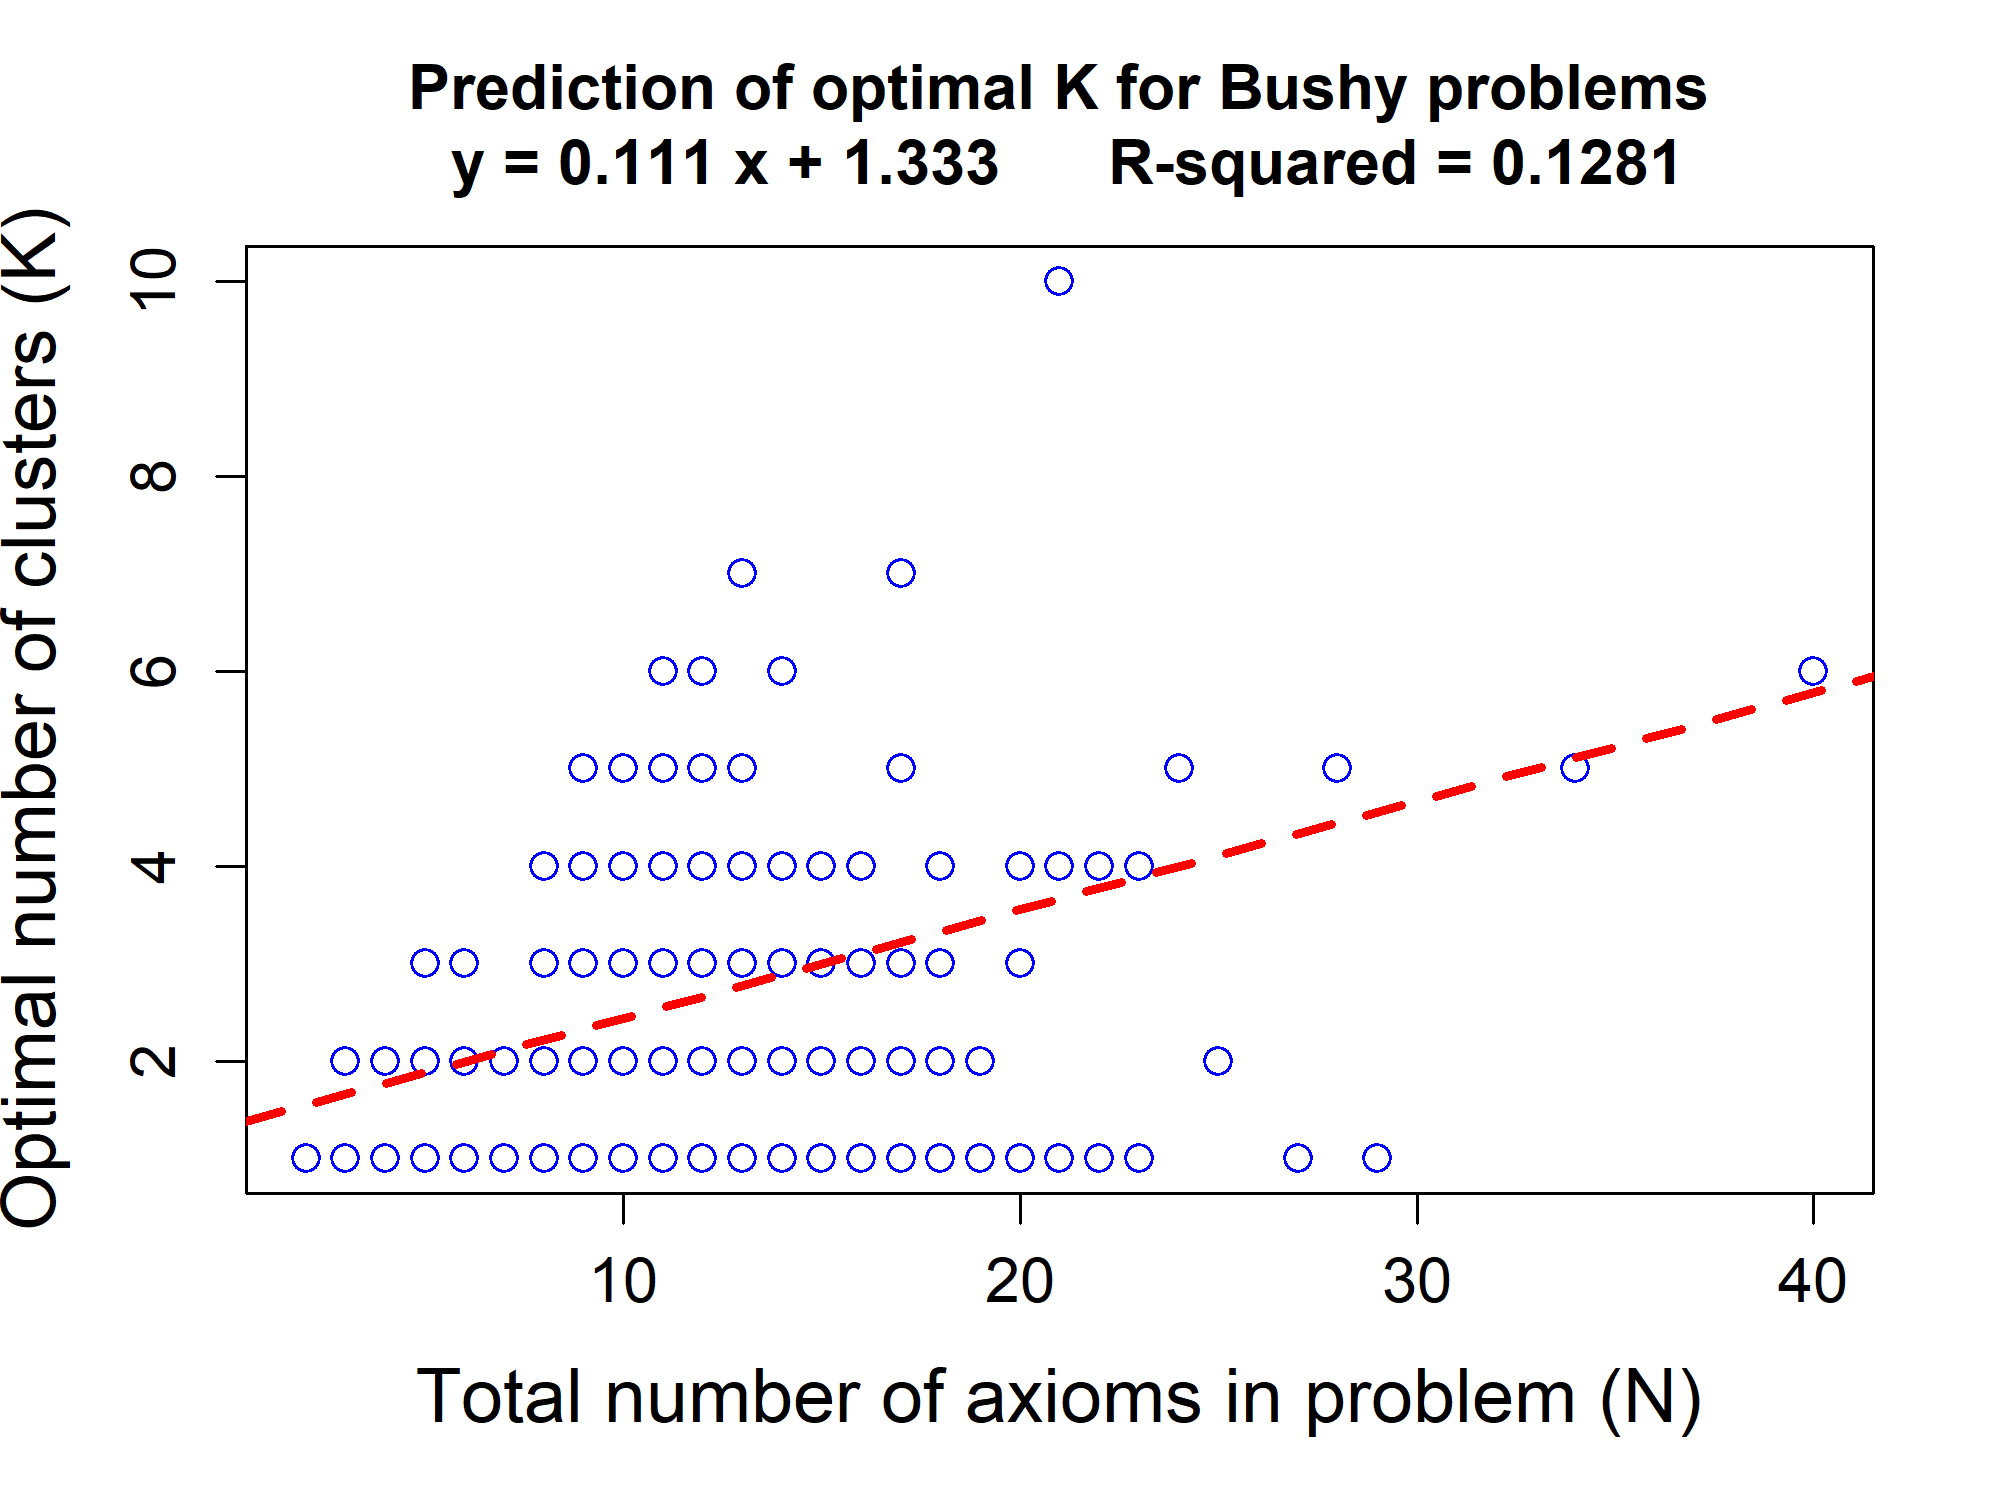
\includegraphics[scale=0.42]{median-regression-optimal-k-bushy.png}
	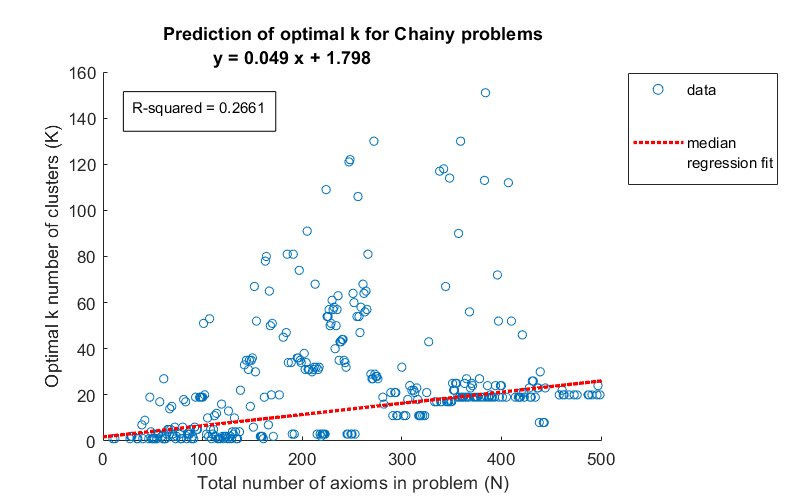
\includegraphics[scale=0.42]{median-regression-optimal-k-chainy.png}
	\vspace{1mm}
	\caption{ Median regression prediction line of $k_{best}$ as a function 
	of the total number of axioms in a problem, for Bushy problems (left) 
	and Chainy problems (right). }
	\label{fig:median-regression}
\end{figure}

%------------------------------------------------------------------------------
\section{Evaluation Results}
\label{Results}

Section on evaluation
1. The test set(s)... Should we add tptp based set?
2. The results
3. The conclusions

Data on MPTPTP2078, Number of problems in test set, how selected (proofs,
hence already solved, but possibly with axiom selection), numbers of
different adequate subsets, average ratio nntp/all

%------------------------------------------------------------------------------
\section{Conclusion}
\label{Conclusion}

GEOFF:
1. Future correlate metrics with ptover performance (or do now!)

%------------------------------------------------------------------------------
\label{sect:bib}
\bibliographystyle{plain}
\bibliography{Bibliography}
%------------------------------------------------------------------------------
\end{document}
%------------------------------------------------------------------------------

